IMSIL supports 1-D, 2-D, and 3-D geometries for static simulations, 
and currently 1-D geometries for dynamic simulations. 
Static simulations may also use rotational symmetry to simplify geometry 
definition and/or improve statistics. 
Geometry is always defined in the target coordinate system.

Like the materials, the geometry can either be defined by \textbf{regions} 
of homogeneous material or by atom densities in \textbf{cells} arranged 
in a regular grid (see Section \ref{s:mater}). 
Homogeneous material regions can be defined using interface positions (1-D), 
polygons (2-D), or signed-distance functions (2-D or 3-D). 
The geometry defined in one of these ways may be extended in each direction 
of each coordinate axis by specifying a boundary type.

In the following, the term ``interface'' refers to the boundary between two
materials, while ``surface'' refers to the interface between the target
and vacuum. 
The term ``domain'' refers to one of three rectangular bodies (intervals in 
1-D, rectangles in 2-D, cuboids in 3-D): 
The \textbf{geometry domain} is the domain where IMSIL must be able to 
calculate the distance from surfaces and interfaces after boundary conditions 
have been applied.
It is identical to the body that circumscribes the user-defined geometry 
(using one of the options described above) except at free surfaces, where
a thin layer is added (see below).
The \textbf{score domain} is the domain where histograms or cell densities 
are scored or fetched from.
For scores in cells, it is identical to the geometry domain. 
For scores in histograms, it may be identical to the geometry domain or extend 
beyond it, depending on the boundary types. 
The \textbf{simulation domain} is the domain where projectiles are allowed 
to move. 
It may be identical to the score domain or extend beyond it, depending on 
the boundary types. 
``Boundaries'' refer to the boundaries of these domains, and are defined by
coordinates on one of the three axes ($x$, $y$, or $z$).

There are four boundary types: 
\textbf{Free} boundaries assume vacuum beyond the boundary. 
Free boundaries allow ions to enter or leave the target or target atoms to 
be sputtered. 
At a free boundary, the geometry domain must extend beyond the target by (at 
least) a few {\AA}ngstr{\o}ms, adding a vacuum layer. 
This is necessary to allow the movement and scoring of projectiles when 
they are outside the target but still interact with the target. 
If the geometry is defined by a distance function or by cell densities, the 
user is responsible for including such a vacuum layer in their input.  

\textbf{Extending} boundaries assume the target properties at the boundary
to extend infinitely beyond the boundary. 
This means, projectiles may move beyond the boundary, and the properties of 
the target at a point outside the boundary are assumed to be identical to 
the position of the normal projection of the point to the boundary. 
At an extending boundary, the score domain is identical to the geometry domain 
by default, and the simulation domain extends to $\pm$ infinity. 
Scores outside the score domain are lost unless the respective 
\texttt{LEXTEND*} flag is set on the \texttt{\&OUTPUT} record.
If the geometry is defined by a distance function or by cell densities, the 
user is responsible for letting the target reach to the boundary.  

\textbf{Periodic} boundaries assume that the target is periodically repeated 
beyond the boundary. 
If both boundaries along a coordinate axis are periodic, scores are mapped 
into the geometry domain unless the respective \texttt{LEXTEND*} flag is set 
on the \texttt{\&OUTPUT} record. 
The score domain then is identical to the geometry domain, since there are no 
scores outside the geometry domain. 
The simulation domain extends to $\pm$ infinity. 
Note that unless \texttt{LEXTEND*} flags are set, the score results and the
beam can be considered periodically repeated like the geometry.
If the geometry is defined by a distance function or by cell densities, the 
user is responsible for letting the target reach to the boundary.  

Finally, \textbf{reflective} boundaries reflect the geometry about the 
boundary. 
The original geometry and its mirror image are treated as if both
were specified in the input file.
The reflection also maps the boundary at the opposite side of the 
reflective boundary to the ``reflected-to" side.
This creates a new boundary at the ``reflected-to'' side of the same type
as the one at the ``reflected-from'' side.
Thus, the new structure has the same boundary type on both sides, and the 
rules for this boundary type apply to both sides.
If the geometry is defined by a distance function or by cell densities, the 
user is responsible for letting the target reach to the boundary.  

Boundary types may be arbitrarily combined along different coordinate axes. 
On opposite sides along the same coordinate axis, a free or extending and 
a periodic boundary or two reflective boundaries may not be combined.
Unless the ions are started from inside the target, there must be at least 
one free boundary that may be hit by the beam.   

\begin{figure}[htbp]
\centering
\noindent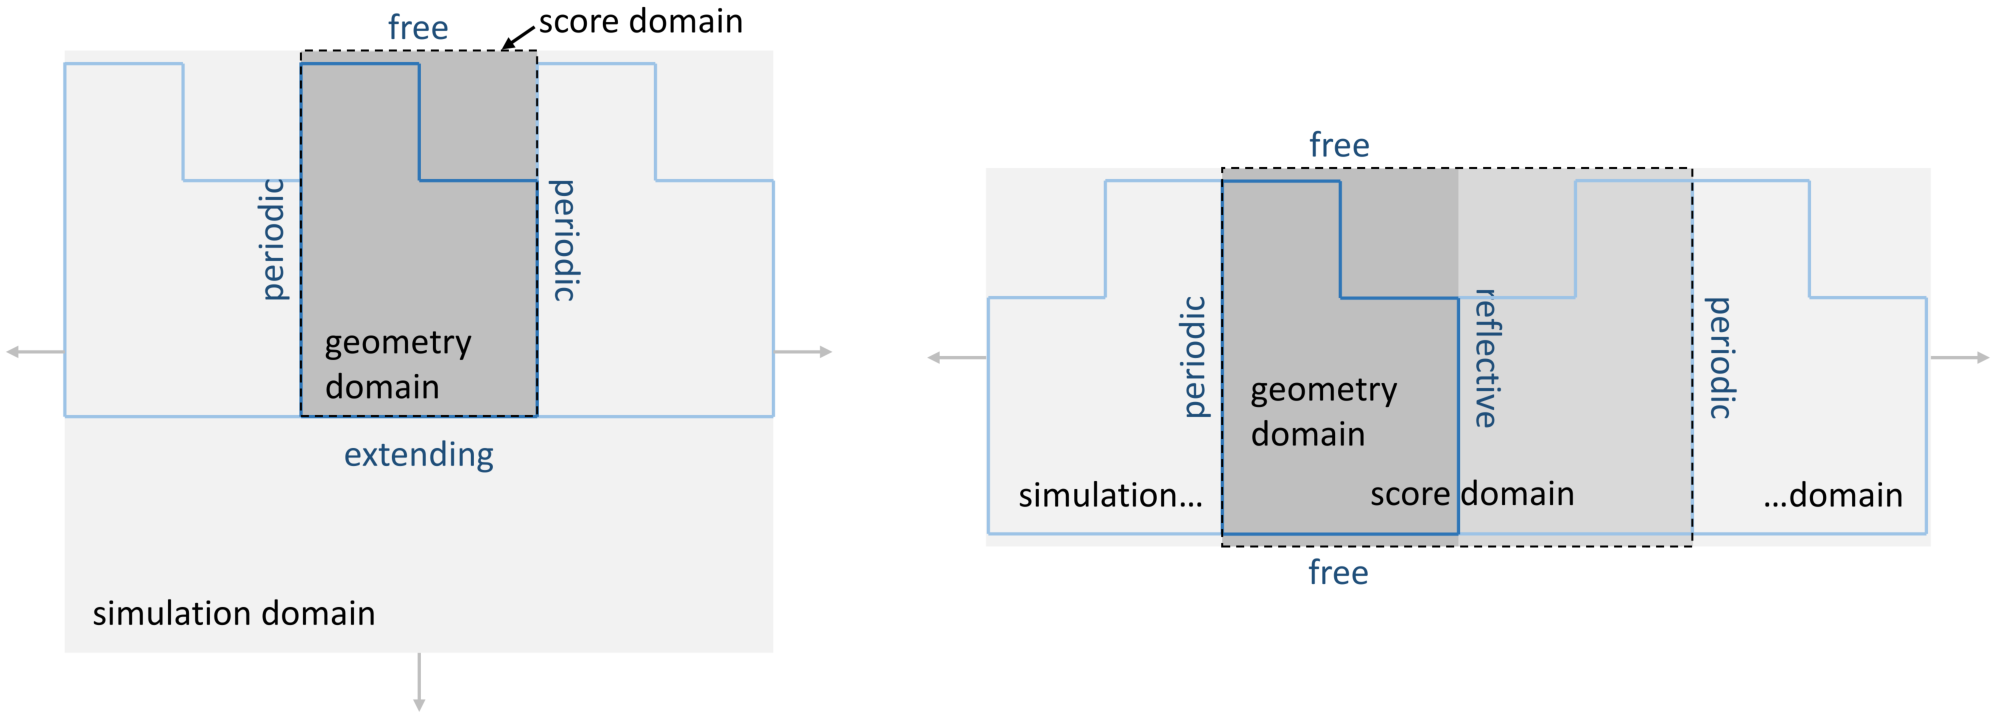
\includegraphics[width=\textwidth]{bndtypes-crop.pdf}
\caption{Examples of geometries. 
The geometry and boundary types on the left represent a semi-infinite target 
with a periodic grating at the top surface.
The geometry and boundary types on the right represent a membrane with a
periodic grating on the top surface, where the grating has a mirror
symmetry. 
The periodic boundary on the right is inferred from mirroring the periodic
boundary on the left about the reflective boundary.
The geometry as specified in the input file is indicated by the dark blue
polygon, while the mirror and periodic images are drawn in light blue.
The geometry domain is indicated by the dark gray rectangle, the score
domain by the mid-gray, and the simulation domain by the light-gray area.}
\label{fig:bndtypes}
\end{figure}
%
Two examples illustrating the boundary types for a 2-D geometry are given in 
Fig.~\ref{fig:bndtypes}.
In the left part of the figure, both lateral boundaries are periodic, the top
boundary is free, and the bottom boundary is extending.
The dark blue polygon represents the geometry as defined in the input file.
Because of the periodic boundaries the geometry is repeated periodically 
on both sides (light blue polygons).
The dark gray rectangle is the geometry domain.
It circumscribes the polygon.
The score domain extends beyond the geometry domain in top direction
by a few {\AA}ngstr{\o}ms, since the top boundary is free.
The projectiles may move anywhere except beyond the free surface position
(light gray region).
The \texttt{LEXTEND*} flags are assumed not to be set, so scores beyond the 
periodic boundaries are mapped into the geometry domain, and scores beneath 
the extending boundary are ignored.
The score domain therefore is identical to the geometry domain except at the
free boundary.

In the example depicted in the right part of Fig.~\ref{fig:bndtypes}, there 
are free boundaries on both the top and bottom of the target.
It therefore represents a membrane.
The grating on the top is periodic, while the period has mirror symmetry.
It is therefore sufficient to specify one half of the structure (dark blue
polygon) with a periodic boundary on one side and a reflective boundary on
the other side.
Again, it is assumed that no \texttt{LEXTENDX} flag is set, so the score 
domain covers the period, while the geometry domain is restricted to one 
half of the period.
The projectiles may move anywhere in lateral direction, but only a few
{\AA}ngstr{\o}ms beyond the minimum and maximum coordinates of the
geometry in vertical direction.

\textbf{1-D geometries} describe layered targets with surfaces and interfaces
parallel to the $x$-$y$ plane. 
They are therefore defined by an array of $z$ coordinates which correspond to 
the positions of the top surface, any interfaces between layers (regions), 
and the bottom surface. 
Semi-infinite and infinite targets may be described by extending boundary 
types in $z$ direction, or may be approximated by large enough values of the 
surface coordinates. 

1-D geometries combined with \textbf{cylindrical or spherical symmetry} 
describe targets composed of cylindrical or spherical shells. 
The surface and interface positions then refer to the distance from the 
symmetry line or center. 
The ``top'' surface is the inner surface, and the ``bottom'' surface the 
outer surface. 
If a hollow body is not desired, the position of the inner surface has
to be assigned a zero or negative value.

During a \textbf{dynamic simulation}, the cell densities are allowed to change
until some threshold is reached for the deviation from equilibrium. 
Then the cell geometries are adapted so that the densities relax towards 
equilibrium. 
For further details see Section~\ref{s:updates}.

\textbf{2-D geometries} are defined in the $x$-$z$ plane, and the geometry 
is assumed to have no variation in $y$ direction.
If polygons are used, they are defined by vertices and their connectivity 
(for details see Section~\ref{s:geom}). 
Since these specifications can be lengthy, they can be put into a separate 
geometry file. 
Internally, the geometry information is converted to a signed distance 
function array for each region. 
The distance values are defined on a regular mesh covering the respective 
region.

\textbf{3-D rotational symmetric geometries} may be realized by combining 2-D
geometries with cylindrical symmetry. 
The symmetry axis can be parallel to the $x$, $y$, or $z$ direction.
If parallel to the $x$ axis, the 3-D geometry is defined by rotating the 
polygons about this axis.
Other orientations of the symmetry axis are realized by permutations of $x$,
$y$, and $z$ \cite{bradley_second_2021}.

Arbitrary 2-D and 3-D geometries may also be defined by \textbf{signed 
distance functions} (SDFs).
The SDFs must be defined on a regular grid and provided as external 
input on files. 
One SDF file per region must be provided.
An SDF value at a grid point specifies the distance of the point from the 
nearest point on the boundary of the region under consideration. 
It is assigned a negative sign when the grid point is outside the region. 
An SDF must also be provided for the whole simulation domain (= the union of 
all regions) including, at free boundaries, a rim of thickness (at least) 
slightly larger than the maximum impact parameter.
For the SDFs, surface segments on extending and reflective boundaries must
not be taken into account nor surface segments shared by both boundaries if 
both boundaries along the axis are periodic. 
All region SDFs must provide values on the whole simulation domain. 
Currently, the user is responsible for the consistency of the SDFs among each
other and with the boundary types.

For surfaces, a simple \textbf{roughness model} is provided. 
This density gradient model \cite{lindsey_simple_2017} reduces the target 
density linearly in space towards the surface in a sub-surface layer. 
The model has been introduced to provide more realistic sputter yields at 
glancing ion incidence. 


\begin{center}
\begin{tabular}{lll}
parameter \quad                   & IMSIL name    & to be specified in record \\
\hline
number of regions                 & \texttt{NR}       & \texttt{\&SETUP} \\
dimensionality                    & \texttt{NDIM}     & \texttt{\&SETUP} \\
1-D surface/interface coordinates & \texttt{POSIF}    & \texttt{\&GEOMETRY} \\
cylindrical symmetry flags        & \texttt{LCYLX}    & \texttt{\&GEOMETRY} \\
                                  & \texttt{LCYLY}    & \texttt{\&GEOMETRY} \\
                                  & \texttt{LCYLZ}    & \texttt{\&GEOMETRY} \\
spherical symmetry flag           & \texttt{LSPHER}   & \texttt{\&GEOMETRY} \\
position of symmetry line/center  & \texttt{CENTER}   & \texttt{\&GEOMETRY} \\
cell-based input flag             & \texttt{USECELL}  & \texttt{\&SETUP} \\
file containing cell densities    & \texttt{CELLFILE} & \texttt{\&SETUP} \\
2-D geometry file                 & \texttt{GEOMFILE} & \texttt{\&GEOMETRY} \\
polygon vertices                  & \texttt{POS}      & \texttt{\&GEOMETRY} \\
polygon connectivity              & \texttt{POINTS}   & \texttt{\&GEOMETRY} \\
boundary types                    & \texttt{BNDTYPEX} & \texttt{\&GEOMETRY} \\
                                  & \texttt{BNDTYPEY} & \texttt{\&GEOMETRY} \\
                                  & \texttt{BNDTYPEZ} & \texttt{\&GEOMETRY} \\
limits of the geometry domain     & \texttt{XLIM}     & \texttt{\&GEOMETRY} \\
                                  & \texttt{ZLIM}     & \texttt{\&GEOMETRY} \\
score extension flags             & \texttt{LEXTENDX} & \texttt{\&OUTPUT} \\
                                  & \texttt{LEXTENDY} & \texttt{\&OUTPUT} \\
                                  & \texttt{LEXTENDZ} & \texttt{\&OUTPUT} \\
box width of distance grid        & \texttt{WBOX2}    & \texttt{\&GEOMETRY} \\
maximum size of distance grid     & \texttt{NBOX2}    & \texttt{\&GEOMETRY} \\
signed distance function file     & \texttt{SDFFILE}  & \texttt{\&GEOMETRY} \\
thickness of roughness layer      & \texttt{WROUGH}   & \texttt{\&GEOMETRY} \\

\end{tabular}
\end{center}

